\documentclass[tikz,border=2pt]{standalone}
\usetikzlibrary{arrows.meta,positioning,calc}
\definecolor{paper}{HTML}{EFE8D8}
\definecolor{ink}{HTML}{2B2A28}
\definecolor{ground}{HTML}{D9CDB2}
\definecolor{muted}{HTML}{6B6457}
\definecolor{cond}{HTML}{3E4A89}
\definecolor{act}{HTML}{7A5618}
\input{/Users/samgilson/Documents/vagrancy/analysis/trees/icons.tex}
\begin{document}
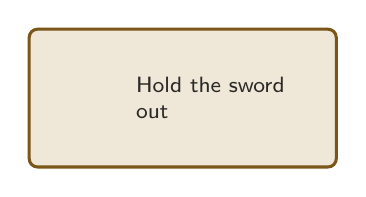
\begin{tikzpicture}[font=\sffamily,
  box/.style={draw, line width=1.1pt, rounded corners=3pt, minimum width=3.9cm, minimum height=1.75cm},
  comp/.style={draw=ink, fill=ground}, cond/.style={draw=cond, fill=paper}, act/.style={draw=act, fill=paper},
  srch/.style={draw=cond, fill=paper, line width=2pt},
  label/.style={anchor=west, text=ink, text width=2.30cm, align=left, font=\sffamily\footnotesize, inner sep=0pt},
  edge/.style={draw=muted, line width=1pt}]
% --- Nodes ---
\node[box, act] (n0) at (1.950,-0.875) {};
\begin{scope}[shift={(0.250,-1.350)}, x=0.0950cm, y=0.0950cm]\def\IC{ink}\def\IW{0.7pt}\IconGuard\end{scope}
\node[label] at (1.350,-0.875) {Hold the sword out};
% --- Edges (after the nodes they join; they end at the borders) ---
\end{tikzpicture}
\end{document}
